\documentclass[unicode,12pt]{beamer}
\usetheme[progressbar=frametitle]{metropolis}    %プレゼンのテーマ設定

%if want to use pdfLatex, specify \iffalse to preamble for LuaLatex and XeLatex
%--------------- preamble for LuaLatex ------------------%

\iffalse
\usepackage{luatexja}
\usepackage[ipaex]{luatexja-preset}
\renewcommand{\kanjifamilydefault}{\gtdefault}
\setsansfont{Calibri}
\fi

%-----------------------------------------------------%

%--------------- preamble for XeLatex -------------------%

\iftrue
\usepackage{xltxtra}
\XeTeXlinebreaklocale "ja"
\usepackage{zxjatype}
\setCJKmainfont[]{Meiryo}
\setsansfont[Scale = 1.1]{Calibri}  % or Arial (Scale = 1)
\fi

%-----------------------------------------------------%

%--------------- general preamble -----------------------%

\definecolor{Cerulean blue}{rgb}{0.16, 0.32, 0.75}
\definecolor{darkcerulean}{rgb}{0.03, 0.27, 0.49}
\definecolor{skyblue}{rgb}{0.4, 0.6, 1.0}
\definecolor{lightpink}{rgb}{1.0, 0.8, 0.76}  %for block color
\definecolor{gray}{gray}{0.8}

\setbeamertemplate{blocks}[default] % Blockの影を消す
%\setbeamertemplate{items}[default] % 箇条書きをシンプルに
\setbeamertemplate{navigation symbols}{} % ナビゲーションシンボルを消す
\setbeamertemplate{footline}[frame number] % フッターはスライド番号のみ
\setbeamertemplate{itemize item}[circle]
\setbeamertemplate{itemize subitem}{--}
\setbeamercolor{frametitle}{bg=skyblue} %or Cerulean blue
\setbeamercolor{title}{fg=darkcerulean}

\iffalse
\usebackgroundtemplate{
    \includegraphics[width=\paperwidth,height=\paperheight]{beamer_background1.pdf}
}
\fi

\usepackage{color}


\newcommand{\emphasis}[2][red]{{\bf{\color{#1} #2}}}
\newcommand{\caveat}[2][blue]{{\bf{\color{#1} #2}}}
\newcommand{\fpartial}[3][\partial]{\frac{#1 #2}{#1 #3}}
\newcommand{\hpartial}[4][\partial]{\frac{#1^{#2} #3}{#1 #4^{#2}}}

\newcommand{\dlinecell}[1]{\begin{tabular}{@{}c@{}} #1 \end{tabular}}

\def\argmax{\text{arg} \max}
\def\argmin{\text{arg} \min}

%-----------------------------------------------------%

\title{Literature Review Workshop in 2020}
\subtitle{}
\author{Hiroki Kato}
\date{May 15, 2020}

\begin{document}

    \maketitle

    \begin{frame}
        \frametitle{参加ありがとうございます}
    
        本ワークショップの開催経緯は、\textbf{単純に私が論文を読むためのコミットメントデバイスが欲しかったから}です。
        
        皆さんも何かしらの意義をこのワークショップに見出してくれたら幸いです。
    
    \end{frame}

    \begin{frame}
        \frametitle{ワークショップのルール}
    
        \begin{itemize}
            \item レビューする分野は不問。なんでもあり。ただし、詳細な実証分析がなされているものに限る
            \item 雑誌レベルもそこまで制限しません(なるべくハイランクであることを望む)。
            \item 発表のためのハンドアウトの作成は任意。ただし、サマリーペーパーはXeLatexを使って、書いてください。研究会の成果として財産にしたいです。
            \begin{itemize}
                \item 書き方の説明をします
            \end{itemize}
            \item 開催は基本zoomです。いつか対面でできる日を祈っています。
            \begin{itemize}
                \item zoomのIDとパスワードはすべて加藤が作成します。
            \end{itemize}
        \end{itemize}
    
    \end{frame}

    \begin{frame}
        \frametitle{SlackとDropbox}
    
        \begin{itemize}
            \item 発表前日までに論文はslackで共有してください。
            \item 論文はDropboxにも保存しておいてくれると助かります(容量がでかくなったら、削除する予定です)。
        \end{itemize}
    
    \end{frame}

    \section{The Hidden Costs of Control}

    \begin{frame}
        \frametitle{}
    
        \centerline{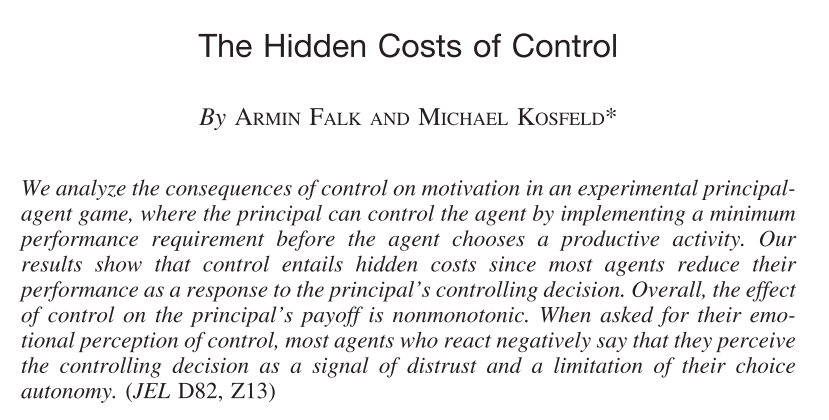
\includegraphics[width = 1.0\linewidth]{0515kato_fig/title.png}}
    
    \end{frame}

    \begin{frame}
        \frametitle{Introduction}
    
        \begin{itemize}
            \item Critical problem of principal-agent relations is \textbf{a conflict of interest}.
            \begin{itemize}
                \item effort $x \in \mathbb{R}_+$ is costly to the agent, and the principal's payoff is increasing in effort $x$.
                \item In standard economics, the agent will choose $x = 0$, which leads to the lowest payoff of the principal.
            \end{itemize}
            \item Two common ways to eliminate agents' actions against a principal's interest.
            \begin{enumerate}
                \item Restrict agent's choice set: $x \in [\underline{x}, +\infty)$
                \item Incentivize agents to take actions following a principal's interest: the agent's payoff is $\pi_A(x) = bx - C(x)$ where $b > 0$.
            \end{enumerate}
        \end{itemize}
    
    \end{frame}

    \begin{frame}
        \frametitle{Introduction}
    
        This paper proposes that \textbf{agents who are intrinsically motivated to perform the principal's interest may decrease performance by control because they perceive control as a negative signal of distrust (control aversion)}.
    
    \end{frame}

    \begin{frame}
        \frametitle{Introduction}
    
        \begin{itemize}
            \item A laboratory experiment which is that the principal can force the agent to choose at least a minimum effort level before the agent chooses effort level.
            \begin{itemize}
                \item Finding 1: A majority of the agents choose a lower effort $x$ if the principal restricts rather than trusts them.
                \item Finding 2: The net effect on profits is non-monotonic, that is, control generates significantly lower profits than trust for low levels of $\underline{x}$, while control breaks even for high levels of $\underline{x}$. 
            \end{itemize}
        \end{itemize}
    
    \end{frame}

    \begin{frame}
        \frametitle{Experimental Design}
    
        \begin{table}[h]
            \footnotesize
            \centering
            \begin{tabular}{c|ccc}
                \hline
                & 
                Principal's choice & 
                Agent's choice &
                N\\
                \hline
                C5  &
                $\underline{x} \in \{0,5\}$ & 
                \dlinecell{$x \in \{\underline{x}, \ldots, 120\}$ in each $\underline{x}$ \\ before learning $\underline{x}$} &
                140 \\
                C10 & 
                $\underline{x} \in \{0,10\}$ & 
                \dlinecell{$x \in \{\underline{x}, \ldots, 120\}$ in each $\underline{x}$ \\ before learning $\underline{x}$} &
                144 \\
                C20 &
                $\underline{x} \in \{0,20\}$ &
                \dlinecell{$x \in \{\underline{x}, \ldots, 120\}$ in each $\underline{x}$ \\ before learning $\underline{x}$} &
                134 \\
                SR10 & 
                $\underline{x} \in \{0,10\}$ & 
                $x \in \{\underline{x}, \ldots, 120\}$ after learning &
                246 \\
                EX10 &
                no decision &
                $x \in \{10, \ldots, 120\}$ &
                72 \\
                GE10 &
                \dlinecell{$\underline{x} \in \{0,10\}$ and \\ $w \in \{10, 30, 60, 120\}$} &
                \dlinecell{$x \in \{\underline{x}, \ldots, 120\}$ in each $(\underline{x}, w)$ \\ 
                           before learning $(\underline{x}, w)$} &
                68 \\
                \hline
            \end{tabular}
        \end{table}
    
    \end{frame}

    \begin{frame}
        \frametitle{Experimental Design}
    
        \begin{itemize}
            \item Payoff functions
            \begin{itemize}
                \item C5, C10, C20, SR10 and EX10: $\pi_p = 2x$ and $\pi_a = 120 - x$
                \item GE10: $\pi_p = 2x - w$ and $\pi_a = w - x$.
            \end{itemize}
            \item Other features of the design
            \begin{itemize}
                \item Timing of decision: (i) principal's choice, (ii) agent's choice
                \item Each principal-agent game was played one-shot.
                \item Subjects were randomly allocated a role as principal or as agent upon arrival at the lab.
            \end{itemize}
        \end{itemize}
    
    \end{frame}

    \begin{frame}
        \frametitle{What We Want to Focus}
    
        \begin{itemize}
            \item C5, C10, and C20: Control aversion by strategy method. The net effect of control on the principal's benefit.
            \item C10 vs EX10: Control aversion predicts that $x$-choices should be higher in the EX10 than in the C10 (Outcome-based preference predicts no difference).
            \item C10 vs SR10: By strategy method, the agents may understate (overstate) their dislike for control.
            \item C10 vs GE10: In the standard social-preference, effort $x$ increases as wage $w$ increases. For higher wages, control may not be optimal since the principal can signal his trust by not choosing control.  
        \end{itemize}
    
    \end{frame}

    \begin{frame}
        \frametitle{Main Result of Agent's Decision}
    
        \centerline{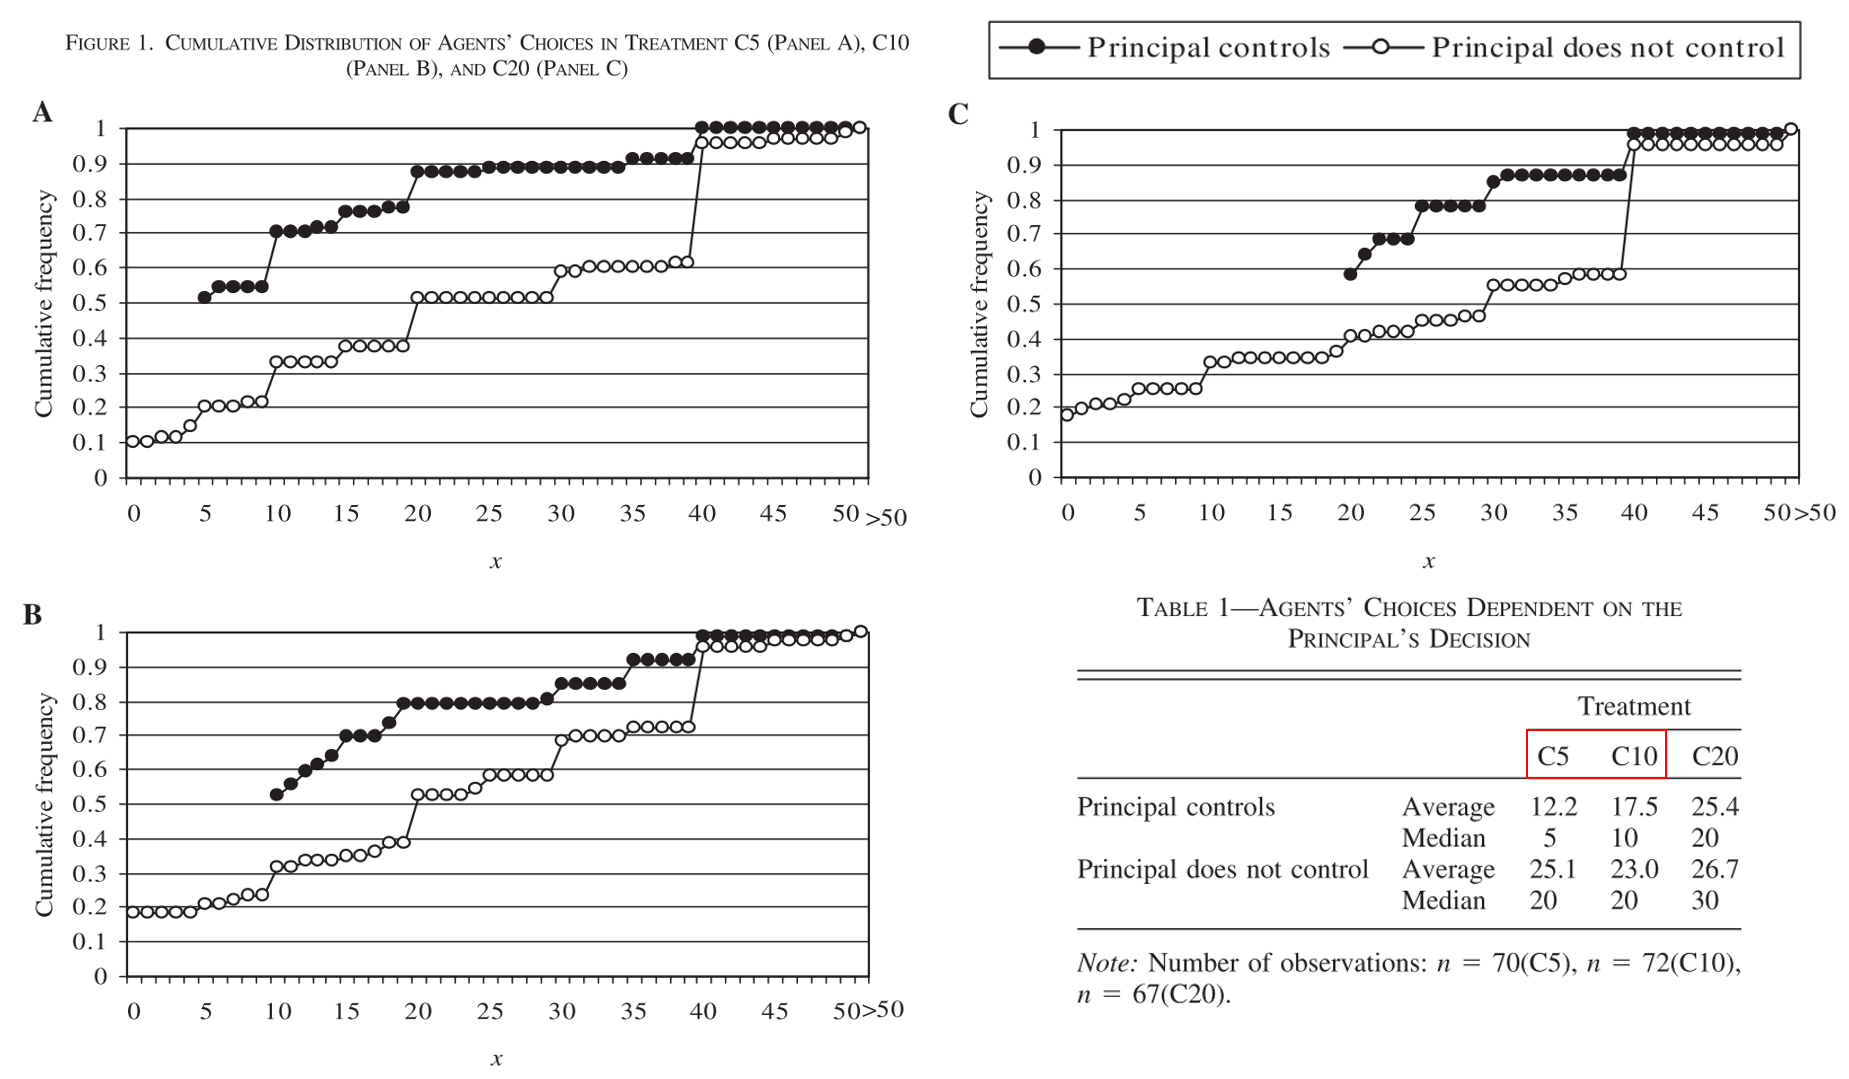
\includegraphics[width = 1.0\linewidth]{0515kato_fig/result1.pdf}}
    
    \end{frame}

    \begin{frame}
        \frametitle{Result 1}
    
        \metroset{block = fill}
        \setbeamercolor{block title}{bg = lightpink}
        \begin{block}{Main Result of Agent's Decision}
            We observe the hidden costs of control in all main treatments. Average performance is higher if the principal does not control than if he does so. These differences are significant in the C5 and the C10, but not in the C20
        \end{block}
        \begin{itemize}
            \item Agents seem to punish the principal's decision to control rather than reward his decision to trust.
        \end{itemize}
    
    \end{frame}

    \begin{frame}
        \frametitle{Heterogeneity of Agent's Decision-Making}
    
        \centerline{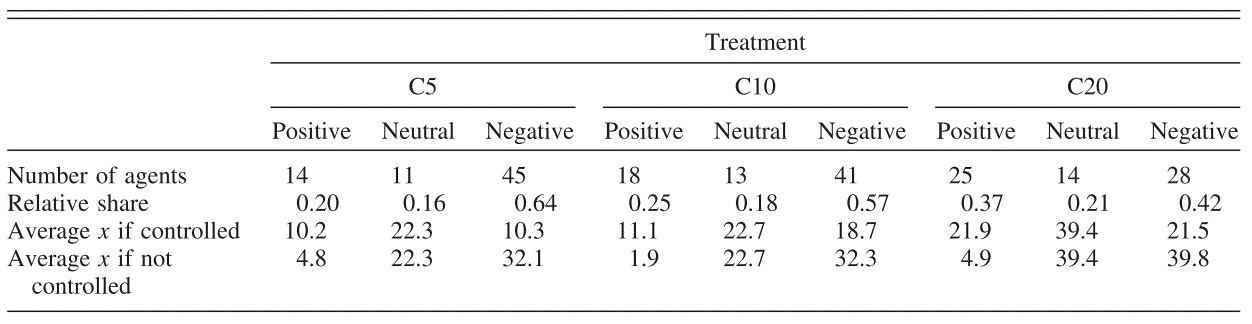
\includegraphics[width = 1.0\linewidth]{0515kato_fig/result2.png}}
    
    \end{frame}

    \begin{frame}
        \frametitle{Result 2}
    
        \metroset{block = fill}
        \setbeamercolor{block title}{bg = lightpink}
        \begin{block}{Heterogeneity of Agent's Decision-Making}
            There is a strong heterogeneity among the agents in all main treatments. We see agents who react positively, neutrally, or negatively to the principal's implementation of control. The last group is always the majority
        \end{block}
        \begin{itemize}
            \item This result shows that the costs of control are substantial. However, this does not suggest that trust is always better than control.
            \item The difference in average profits between controlling and trusting is -25.8 in C5, -11.0 in C10, and -2.6 in C20.
        \end{itemize}
    
    \end{frame}

    \begin{frame}
        \frametitle{Robustness Check}
    
        \begin{itemize}
            \item Robustness 1: There is no any effect of using the strategy method versus the specific response method.
            \item Robustness 2: $x$-choices in the EX10 treatment exceed those in the C10 subgame following the control decision.
            \item Robustness 3: Agents who are controlled think that the principal has lower expectations than do agents who are not controlled in the SR10 treatment.
            \item Robustness 4: most agents who reacted negatively to control in the experiment felt distrust and lack of autonomy.
        \end{itemize}
    
    \end{frame}

    \begin{frame}
        \frametitle{Behavior and Beliefs of Principals}
    
        \centerline{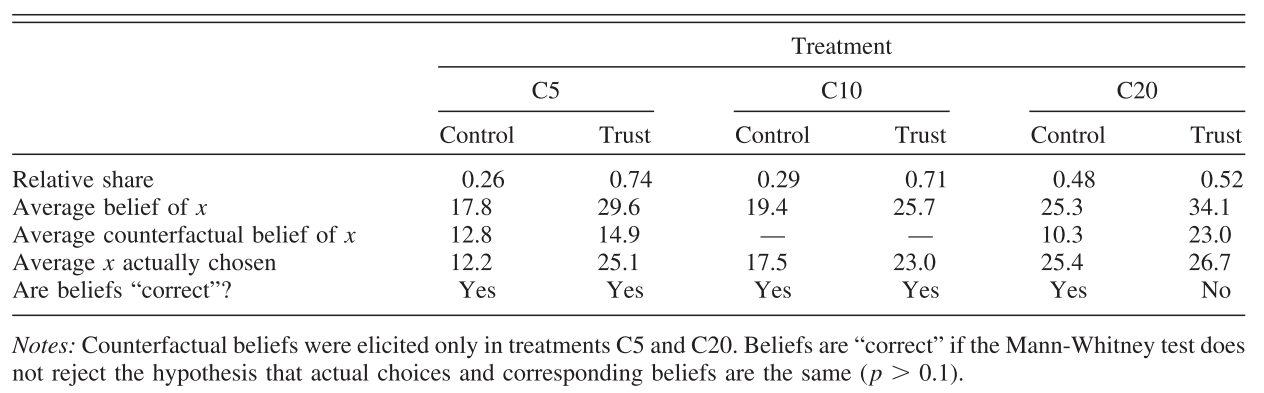
\includegraphics[width = 1.0\linewidth]{0515kato_fig/result3.png}}
    
    \end{frame}

    \begin{frame}
        \frametitle{Result 3}

        \metroset{block = fill}
        \setbeamercolor{block title}{bg = lightpink}
        \begin{block}{Behavior and Beliefs of Principals}
            There is a strong heterogeneity among the agents in all main treatments. We see agents who react positively, neutrally, or negatively to the principal's implementation of control. The last group is always the majority
        \end{block}
        \begin{itemize}
            \item Self-fulfilling prophecy of distrust: \textit{Principals who have rather pessimistic beliefs and hence choose to restrict the agent's choice set experience that their beliefs are indeed confirmed by their agents' relatively low average performance}.
        \end{itemize}
    
    \end{frame}

    \begin{frame}
        \frametitle{Results of GE10 Treatment}
    
        \centerline{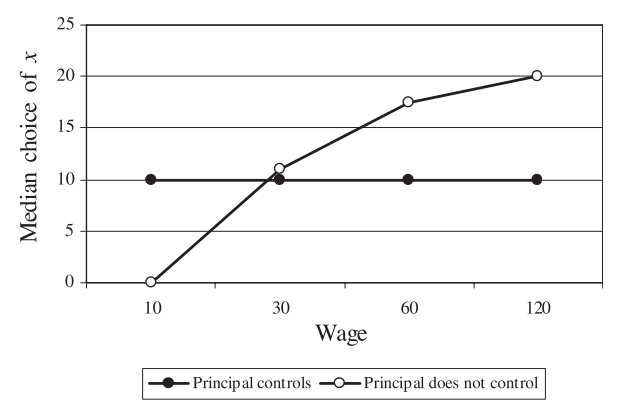
\includegraphics[width = 1.0\linewidth]{0515kato_fig/result4.png}}
    
    \end{frame}

    \begin{frame}
        \frametitle{Result 4}
    
        \metroset{block = fill}
        \setbeamercolor{block title}{bg = lightpink}
        \begin{block}{Results of GE10 Treatment}
            We observe reciprocity in the gift-exchange treatment, i.e., a positive relationship between wages and effort. Reciprocity is significantly weaker, however, if the principal controls than if he does not control
        \end{block}
        \begin{itemize}
            \item The net benefits of control are decreasing in wages, i.e., the negative effect of control on reciprocal agents is slightly stronger than the positive effect of control on selfish agents.
        \end{itemize}
    
    \end{frame}

    \begin{frame}
        \frametitle{Concluding Remarks}
    
        \begin{quote}
            The main message of our paper is that control and explicit incentives entail hidden costs,
            which should be taken seriously.
            The message is \textit{not}, however, that it is always better for principals to trust than to control.
            In fact, we show that the costs and benefits of controlling agents depend on various factors.
            First, they depend on the composition of agents' type.
            \dots
            Second, the strength of the explicit incentives is important (Falk and Kosfeld, 2006, p.1628).
        \end{quote}
    
    \end{frame}

\end{document}